\documentclass[]{article}
\newcommand{\FileDepth}{../..}
\usepackage[a4paper, total={15cm,23cm}]{geometry}
\usepackage[T1]{fontenc}
\usepackage{textcomp}%Not strictly necessary, but gives \textmu command for "micro."
\usepackage{fancyhdr}
\usepackage{amsmath}
\usepackage{amssymb}
\usepackage{graphicx}
\usepackage{xcolor}
\usepackage{tikz}
\usetikzlibrary{calc}
\usepackage{cancel}
%opening
\newcommand{\SecType}{X}
\newcommand{\Week}{X}
\title{Springloaded Sled}
\author{Benjamin Bauml}
\date{Summer 2024}
\pagestyle{fancy}
\rhead{PH 211}
\chead{Summer 2024}
\lhead{Week \Week}

% For Assignment, leave Purpose as 1. For Worksheet, set to 2. For Student Solution, set to 3. For Teacher Solution, set to 4.
% If you want keep the pieces from being called manually, set DefOnly to 0.
\newcommand{\Purpose}{4}
\newcommand{\DefOnly}{1}

% Version 2024-06-14
% Changes
% 2024-02-21 Added xstring package to enable smooth implementation of new \ModePage command.
% 2024-04-27 Set up to split activities and formatting aspects into separate files. Removed dependence on xcomment. Added an automatic counter to number the activities in a problem set.
% 2024-05-19 Revised old format for \TeachingTips command, which did not support \DefOnly.
% 2024-06-14 Added Repurpose environment to allow mixing of different purpose levels in the same document.
\usepackage{tcolorbox}
\usepackage{xstring}
% You will want the following four lines in your document (the last two uncommented):
% For Assignment, leave Purpose as 1. For Worksheet, set to 2. For Student Solution, set to 3. For Teacher Solution, set to 4.
% If you want keep the pieces from being called manually, set DefOnly to 0.
%\newcommand{\Purpose}{4}
%\newcommand{\DefOnly}{1}
\newcommand{\Exclusion}{0}
\newcommand{\PageTurn}{0}
\newcommand{\GrayProb}{0}
\newcommand{\Tipsy}{0}

% Assignment
\if\Purpose1
\renewcommand{\Exclusion}{1}
\fi
% Worksheet
\if\Purpose2
\renewcommand{\Exclusion}{1}
\renewcommand{\PageTurn}{1}
\fi
% Student Solution
\if\Purpose3
\renewcommand{\PageTurn}{1}
\renewcommand{\GrayProb}{1}
\fi
% Teaching Copy
\if\Purpose4
\renewcommand{\PageTurn}{1}
\renewcommand{\GrayProb}{1}
\renewcommand{\Tipsy}{1}
\fi

\newenvironment{Repurpose}[1]{
\renewcommand{\Purpose}{#1}
\renewcommand{\Exclusion}{0}
\renewcommand{\PageTurn}{0}
\renewcommand{\GrayProb}{0}
\renewcommand{\Tipsy}{0}
% Assignment
\if\Purpose1
\renewcommand{\Exclusion}{1}
\fi
% Worksheet
\if\Purpose2
\renewcommand{\Exclusion}{1}
\renewcommand{\PageTurn}{1}
\fi
% Student Solution
\if\Purpose3
\renewcommand{\PageTurn}{1}
\renewcommand{\GrayProb}{1}
\fi
% Teaching Copy
\if\Purpose4
\renewcommand{\PageTurn}{1}
\renewcommand{\GrayProb}{1}
\renewcommand{\Tipsy}{1}
\fi
}{}

\def \NewQ {0}
\def \PForce {0}
\newcommand{\MaybePage}[1]{
	\def \PForce {#1}
	\if\PForce1
	\newpage
	\else
	\if\NewQ0
	\gdef \NewQ {\PageTurn}
	\else
	\newpage
	\fi
	\fi
}

\newcommand{\ModePage}[1]{
	\IfSubStr{#1}{\Purpose}{\newpage}{}
}

\newcounter{ActNumber}
\setcounter{ActNumber}{0}

\newcommand{\Problem}[4][0]{%The first argument is optional, and if it is set to 1, the \newpage will be forced. The second argument is the name of the activity, the third is the command the activity is stored as, and the fourth is the actual problem statement.
\newcommand{#3}{
\MaybePage{#1}
\addtocounter{ActNumber}{1}
\section*{\SecType\Week-\theActNumber: #2}
\if\GrayProb1
\begin{tcolorbox}[colback=lightgray,colframe=lightgray,sharp corners,boxsep=1pt,left=0pt,right=0pt,top=0pt,bottom=0pt,after skip=2pt]
\else
\begin{tcolorbox}[colback=white,colframe=white,sharp corners,boxsep=1pt,left=0pt,right=0pt,top=0pt,bottom=0pt,after skip=2pt]
\fi
#4
\end{tcolorbox}\noindent
}
\if\DefOnly0
\else
#3
\fi
}
	
\newcommand{\ProblemSub}[3][0]{%The first argument is optional, and if a string of numbers is entered into it, it will force a \newpage in any \Purpose that shows up in the string. For example, "13" would lead to the newpage being forced in modes 1 and 3. The second is the command the activity is stored as, and the third is the actual problem statement.
\newcommand{#2}{
\ModePage{#1}
\if\GrayProb1
\begin{tcolorbox}[colback=lightgray,colframe=lightgray,sharp corners,boxsep=1pt,left=0pt,right=0pt,top=0pt,bottom=0pt,after skip=2pt]
\else
\begin{tcolorbox}[colback=white,colframe=white,sharp corners,boxsep=1pt,left=0pt,right=0pt,top=0pt,bottom=0pt,after skip=2pt]
\fi
#3
\end{tcolorbox}\noindent
}
\if\DefOnly0
\else
#2
\fi
}
		
\newcommand{\Solution}[2]{%The first argument is the command the solution is stored as, and the second is the actual solution.
\newcommand{#1}{
\if\Exclusion0
#2
\fi
}
\if\DefOnly0
\else
#1
\fi
}
		
\newcommand{\ProblemFig}[2]{%The first argument is the command the figure is stored as, and the second is the actual figure.
\newcommand{#1}{
\begin{figure}[h]
#2
\end{figure}
}
\if\DefOnly0
\else
#1
\fi
}

\newcommand{\TeachingTips}[2]{%The first argument is the command the tip is stored as, and the second is the actual tip.
\newcommand{#1}{
\if\Tipsy1
\begin{tcolorbox}[colback=lightgray,colframe=black]
#2
\end{tcolorbox}
\fi
}
\if\DefOnly0
\else
#1
\fi
}
\newcommand{\MVec}[3][0]{%Creates a momentum vector of length #3 centered at #2 and rotated #1 degrees counterclockwise.
	\begin{scope}[rotate=#1,shift={(#2)}]
		\draw[->,thick] ({-#3/2},0) -- ({#3/2},0);
	\end{scope}
}
\newcommand{\MDot}[1]{%Creates a dot at #1 to represent a zero vector.
	\filldraw (#1) circle (1pt);
}
\newcommand{\MVDRows}[2][4.5]{%Creates the rows (initial, delta, final) of a momentum vector diagram. The optional argument determines the width of the table, and defaults to a good length for three columns (two objects and the total system). The non-optional argument gives a coordinate name (not displayed) to the diagram.
	\begin{scope}
		%\draw[thick] (0,5.5) -- (0,0);
		\draw[thick] (-1,4.5) -- (#1,4.5);
		\node at (-0.5,3.75) {$\vec{p}_{i}$};
		\draw[thick] (-1,3) -- (#1,3);
		\node at (-0.5,2.25) {$\Delta\vec{p}$};
		\draw[thick] (-1,1.5) -- (#1,1.5);
		\node at (-0.5,0.75) {$\vec{p}_{f}$};
		\coordinate (#2) at (0,5);
	\end{scope}
}
\newcommand{\MVDCol}[4][0.75]{%Creates a column for an object in a momentum vector diagram. The first (non-optional) argument is the coordinate name (not displayed) of the column, while the second is the displayed column header. The first argument also names the three entries down the column. The third argument anchors the column, so it should either be the coordinate name of the MVD (for the first column) or the coordinate name of the previous column. The optional argument indicates how far the center of the column should be from the previous column's edge, and defaults to 0.75
	\begin{scope}[shift={(#4)}]
		\node at (#1,0) {#3};
		%\draw[thick] ({#1*2},0.5) -- ({#1*2},-5);
		\draw[thick] (0,0.5) -- (0,-5);
		\coordinate (#2init) at (#1,-1.25);
		\coordinate (#2delt) at (#1,-2.75);
		\coordinate (#2fin) at (#1,-4.25);
		\coordinate (#2) at ({#1*2},0);
	\end{scope}
}

\begin{document}
\maketitle

\Problem{Springloaded Sled}{\SpringSled}{
You are designing a sled with a compressed spring inside, which can be released to separate the sled into two pieces of equal mass ($m/2$). You are racing the sled across level snow at speed $v$ when you trigger the separation.
%A firework is moving to the right with speed v when it explodes into two pieces with equal mass (m/2).
}
\ProblemSub{\SpringSledMomEn}{
Right after the two halves push apart, the back end of the sled is moving backward with speed $v$. What is the velocity of the other piece? How much kinetic energy did the system gain?
%Right after the explosion, the first piece is moving backward with speed v.
%What is the velocity of the other piece?
%How much kinetic energy did the system gain?
}
\ProblemFig{\SpringSledFig}{
\centering
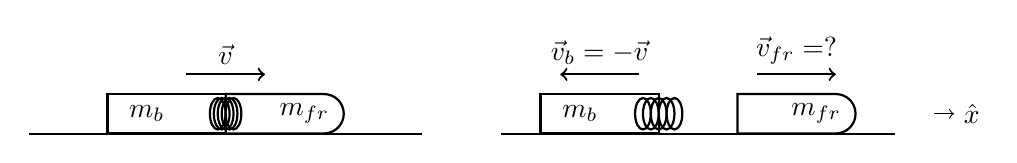
\begin{tikzpicture}
	\begin{scope}[rotate=0,shift={(-3,0)}]
		\draw[thick,->] (-0.5,0.5) -- (0.5,0.5);
		\node[anchor=south] at (0,0.5) {$\vec{v}$};
		\begin{scope}
			\draw[thick] (-1.5,0.25) rectangle (0,-0.25);
			\node at (-1,0) {$m_{b}$};
		\end{scope}
		\begin{scope}
			\draw[thick] (0,0.25) -- (1.25,0.25) arc (90:-90:0.25) -- (0,-0.25) -- cycle;
			\node at (1,0) {$m_{fr}$};
		\end{scope}
		\begin{scope}[yscale=2]
			\newcommand{\Comp}{0.05}
			\draw[thick] ({-\Comp*2},0) circle (0.1);
			\draw[thick] (-\Comp,0) circle (0.1);
			\draw[thick] (0,0) circle (0.1);
			\draw[thick] (\Comp,0) circle (0.1);
			\draw[thick] ({\Comp*2},0) circle (0.1);
		\end{scope}
		\draw[thick] (-2.5,-0.26) -- (2.5,-0.26);
	\end{scope}
	\begin{scope}[rotate=0,shift={(3,0)}]
		\begin{scope}[shift={(-0.5,0)}]
			\draw[thick,->] (-0.25,0.5) -- (-1.25,0.5);
			\node[anchor=south] at (-0.75,0.5) {$\vec{v}_{b}=-\vec{v}$};
			\draw[thick] (-1.5,0.25) rectangle (0,-0.25);
			\node at (-1,0) {$m_{b}$};
		\end{scope}
		\begin{scope}[shift={(0.5,0)}]
			\draw[thick,->] (0.25,0.5) -- (1.25,0.5);
			\node[anchor=south] at (0.75,0.5) {$\vec{v}_{fr}=$?};
			\draw[thick] (0,0.25) -- (1.25,0.25) arc (90:-90:0.25) -- (0,-0.25) -- cycle;
			\node at (1,0) {$m_{fr}$};
		\end{scope}
		\begin{scope}[yscale=2,shift={(-0.5,0)}]
			\newcommand{\Comp}{0.1}
			\draw[thick] ({-\Comp*2},0) circle (0.1);
			\draw[thick] (-\Comp,0) circle (0.1);
			\draw[thick] (0,0) circle (0.1);
			\draw[thick] (\Comp,0) circle (0.1);
			\draw[thick] ({\Comp*2},0) circle (0.1);
		\end{scope}
		\draw[thick] (-2.5,-0.26) -- (2.5,-0.26);
	\end{scope}
	\begin{scope}[shift={(6,0)}]
		\draw[->] (0,0) -- (0.25,0);
		\node[anchor=west] at (0.25,0) {$\hat{x}$};
	\end{scope}
\end{tikzpicture}
}
\Solution{\SpringSledSol}{
	
When setting up a motion vector diagram for this problem, I know the initial momentum of the combined sled system, and I know both parts of the sled have half of this momentum. I also know that the final momentum of the back half is reversed, and the total momentum of the system is unchanged, so I can infer the rest of the table from there.
\begin{figure}[h]
	\centering
	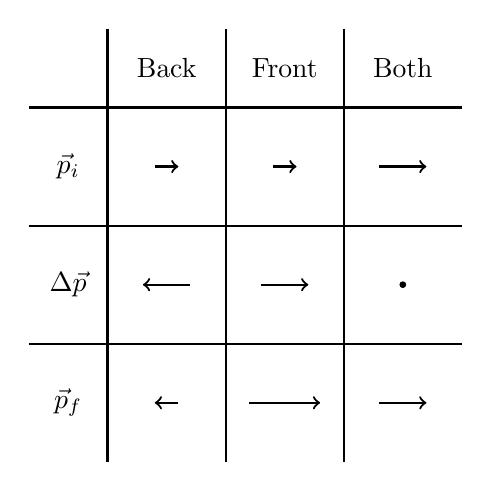
\begin{tikzpicture}
		\MVDRows{MVD}
		\MVDCol{mass}{Back}{MVD}{0.75}
		\MVec{massinit}{0.3}
		\MVec[180]{massdelt}{0.6}
		\MVec[180]{massfin}{0.3}
		\MVDCol{Mass}{Front}{mass}{0.75}
		\MVec{Massinit}{0.3}
		\MVec{Massdelt}{0.6}
		\MVec{Massfin}{0.9}
		\MVDCol{sys}{Both}{Mass}{0.75}
		\MVec{sysinit}{0.6}
		\MDot{sysdelt}
		\MVec{sysfin}{0.6}
	\end{tikzpicture}
\end{figure}

The initial momentum of the system is $mv\hat{x}$, and the final momentum is $(\frac{m}{2}v_{fr}-\frac{m}{2}v)\hat{x}$. Since the momentum is conserved (no friction, and the normal force and gravitational force are in balance, so no other net impulse), we know that
\begin{align*}
	mv\hat{x} & = \left(\frac{m}{2}v_{fr}-\frac{m}{2}v\right)\hat{x} \\
	mv & = \frac{m}{2}v_{fr}-\frac{m}{2}v \\
	2v & = v_{fr} - v \\
	v_{fr} & = 3v.
\end{align*}
The front half of the sled gets launched forward at triple its original speed!

As for kinetic energy, the system started with $K_{i} = \frac{1}{2}mv^{2}$, and now it has
\[
K_{f} = \frac{1}{2}\frac{m}{2}v^{2} + \frac{1}{2}\frac{m}{2}(3v)^{2} = \frac{5}{2}mv^{2},
\]
therefore the change in kinetic energy is
\[
\Delta K = K_{f}-K_{i} = 2mv^{2}.
\]

This came from the spring. If the spring constant is $k$ and the spring was compressed by a length $\Delta x$, then we have
\begin{align*}
\frac{1}{2}k\Delta x^{2} & = 2mv^{2} \\
k\Delta x^{2} & = 4mv^{2}.
\end{align*}
This has some interesting design implications. For example, say each half of our sled is 100 kg (say that accounts for the machinery and the load of a single passenger on each half) and its initial speed was a lazy 1 m/s. That would mean the spring has to store 400 J of energy. If $\Delta x = 0.5$ m (which may be too much of a compression for a reasonable use of Hooke's law), then $k=3200$ N/m (or 32 N/cm), which is a pretty stiff spring. If we cannot get a spring this stiff, then we need more compression, but if we cannot obtain a spring that compresses far enough without permanently deforming, then we need it stiffer. The key will be finding the perfect middle ground (and those of you who are doing experiments with elasticity in your capstone lab might have a better idea than using a single spring).
}
\end{document}